\documentclass[a4paper]{ctexart}
\usepackage[utf8]{inputenc}
\usepackage[a4paper]{geometry}
\usepackage{graphicx}
\usepackage{hyperref}
\usepackage[heading = false]{ctex}
\usepackage{xcolor}
\usepackage{fontspec}
\usepackage{listings}
\pagestyle{plain}
\geometry{top=1.0cm, bottom=2.0cm}
\setmonofont{Cascadia Code PL}
\lstset{
    basicstyle = \ttfamily,
    commentstyle = \itshape,
    numbers = left,
    numberstyle = \zihao{-5}\ttfamily,
    frame = lrtb
}

\begin{document}
  \begin{titlepage}
      \songti
      \begin{center}
        \vspace*{2cm}
        {\fontsize{24pt}{0}
          \textbf{计算机通信与网络\\实验报告\\}
        }
        \vspace*{10cm}
        {\fontsize{16pt}{0}
          \textbf{\ 姓\quad 名\ }: \underline{\makebox[100pt]{xxx}}\\
          \textbf{\ 学\quad 号\ }: \underline{\makebox[100pt]{\large xxxx}}\\
          \textbf{\ 班\quad 级\ }: \underline{\makebox[100pt]{\large xxxx}}\\
          \textbf{上课时间}: \underline{\makebox[100pt]{\large yyyy.mm.dd}}\\
        }
        \vspace*{7cm}
        {\fontsize{16pt}{0}
          \textbf{实验名称: {\Large Coding on error dectecting algorithms}}
        }
      \end{center}
  \end{titlepage}

  \CTEXsetup[format={\Large\bfseries}]{section}

  \newpage
  \section{实验目的}
    \begin{itemize}
      \item Learn CRC principles and master CRC16-IBM writing method
      \item Learn the principle of Parity Check and write it in C
    \end{itemize}

  \section{实验内容与要求}
    \begin{enumerate}
      \item \textbf{Cyclic redundancy check\\}
      Using the polynomials below to encode random generated data stream(40-100bits).
      Show the FEC, and encoded data frame.
      \item \textbf{Parity check\\}
      Using even or odd parity check on random generated data stream (8-20bits).
      Show encoded data frame.
    \end{enumerate}

    \paragraph{实验原理}
    \begin{enumerate}
      \item 在K位信息码后再拼接R位的校验码,整个编码长度为N位。
      \item 对于一个给定的(N,K)码,存在一个最高次幂为R=N-K的多项式G(X),
            根据G(X)可以生成K位信息的校验码。G(X)称为这个CRC的生成多项式。
      \item 将K位信息码左移R位后,与G(X)做模-2除法,得到的R位余数即为校验码。
      \item 将校验码附加到K位信息码后得到(K+R)位的CRC序列作为传输内容
      \item 接收方把接收到的内容与同一个G(X)做模-2除法, 若得到余数为0,则码字无错,
            若有一位出错,余数不为0,且不同的出错位得到不同的余数。
      \item 将余数拼到信息码左移后空出的位置,得到完整的CRC码。
    \end{enumerate}

    \newpage
    \section{实验程序与结果}
    \subsection{运行结果}
    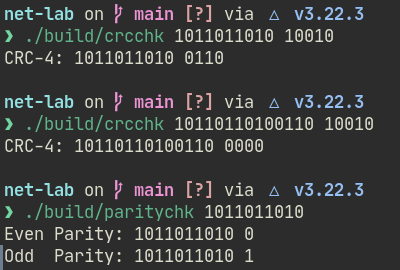
\includegraphics[width=0.7\textwidth]{fig/result.png}
    \subsection{程序代码}
    见\hyperlink{appendix}{附录}

    \section{实验结果分析}
      \subsection*{CRC校验}
      \paragraph{编码}
      由上图可得,要传输的数据为1011011010,使用生成多项式10010得到的CRC-4校验字为0110,
      所以最后的输出结果为10110110100110
      \paragraph{解码}
      由上图可得,将编码结果10110110100110和生成多项式10010输入程序,得到的CRC-4校验字为0000,
      说明校验结果正确

      \subsection*{奇偶校验}
      \paragraph{编码}
      由上图可得,对于输入数据1011011010,奇校验为末尾补1,偶校验为末尾补0
      \paragraph{解码}
      由于输入数据1011011010中有偶数个零,可知校验结果正确

    \newpage
    \section{实验问题解答与体会}
    本实验设计研究了循环冗余校验码的原理,以及利用C++语言对其进行编程仿真,
    得到的结论和理论上是一致的,简单而且快捷。设计过程中查阅了有关CRC设计的书籍,
    巩固了以前所学过的知识,而且学到了很多在书本上所没有学到过的知识。
    通过这次课程设计使我懂得了理论与实际相结合的必要性,只有理论知识是远远不够的,
    只有把所学的理论知识与实践相结合起来,从理论中得出结论,
    从而提高自己的实际动手能力和独立思考的能力。

    \newpage
    \appendix
    \hypertarget{appendix}{}
    \section*{附录}

    \subsection*{共享库}
    \lstinputlisting[language=C++, caption=binutils.h]{code/include/binutils.h}
    \lstinputlisting[language=C++, caption=binutils.cpp]{code/src/binutils.cpp}
    \newpage

    \subsection*{CRC校验}
    \lstinputlisting[language=C++, caption=crcchk.cpp]{code/src/crcchk.cpp}
    \newpage

    \subsection*{奇偶校验}
    \lstinputlisting[language=C++, caption=paritychk.cpp]{code/src/paritychk.cpp}
\end{document}
